We are now ready to present experimental results of \sys performance. We start with describing the hardware environment (Section~\ref{sec:results_hardware}) followed by the software environment (Section~\ref{sec:results_software}) and we concluded by the evaluation results (Section~\ref{sec:results_evaluation}).

\subsection{Hardware Suite Description}
\label{sec:results_hardware}

In all experiments we used the following computing hardware: WISP\,5.1~\cite{wisp5,wisp}, i.e. build around MSP430FR5969~\cite{wolverine} 64\,kB FRAM microcontroller, and TI's MSP430FR5969 launchpad~\cite{MSP-EXP430FR5969_launchpad} (hardware type will be specified per experiment in Section~\ref{sec:results_evaluation}). WISP\,5.1 has been re-programmed during experiments using TI's Flash Emulation Tool (FET)~\cite{fet}. FET was also used as a power supply in non-intermittent power experiment. To measure energy consumption of all benchmark applications (please refer to Section~\ref{sec:results_software}) Carnegie Mellon's EDB~\cite{edb} was used. In experiments involving wireless power, WISP was powered through an RFID reader (Impinj R1000 with firmware version 3.2.4.240~\cite{r1000_data_sheet}) connected to Liard RFMAX S9028PCRJ 8\,dBic~\cite{atlas2015}. RFID reader is controlled by a PC running Ubuntu 10.4 executing open source Python-based \emph{sllurp} library~\cite{sllrp_github} enabling low-level RFID reader control. Transmitted power of the RFID reader was 30\,dBm at 915\,MHz center frequency. For distance controlled experiments, WISP was positioned at varying length hollow paper tubes placed directly on a flat lying antenna. Code completion measurements have been performed using Salea~\cite{saleae} digital logic analyzer.

\subsection{Software Suite Description}
\label{sec:results_software}

We compare \sys against state of the art intermittent execution approach---Chain~\cite{chain}. We are not comparing \sys against DINO~\cite{dino} or Mementos~\cite{mementos} (Refer to Section~\ref{sec:background_consistency}), as (i) Chain is the only modular execution model available to which we can compare \sys, and (ii) Chain proves already its superiority over sequential model counterparts (i.e. DINO and Mementos).

We need to note that although another very relevant task-based runtime has been recently presented and referenced many times throughout this paper---Alpaca~\cite{alpaca} (written by the same group as Chain)---except the recently accepted manuscript we did not have the access to Alpaca's code during the preparation of this paper. Therefore Alpaca was excluded from the evaluation.

\todo{Check if the line of argument is solid for the above paragraphs about not selecting DINO, Memenos and Aplaca}{Brandon}

The applications that were used in the evaluation are given in Table~\ref{table:benchmark_list}. These benchmarks are the same ones as used in~\cite{chain,alpaca}. In addition to Chain benchmark programs new applications were used for benchmarking: \emph{DFT}, \emph{Huffman compressor}, and \emph{selection sort}.

\begin{table}[t]
	\begin{tabular}{|c|c|c|}
		\hline
		Nickname & SLOC (\sys) & SLOC (Chain~\cite{chain})\\
		\hline\hline
		Cold chain & 388 & 721 \\ %53\%
		Cuckoo & 483 & 762 \\ %63\%
		RSA & 887 & 1233 \\ %71\%
		Bitcount & 351 & 588 \\ %59\%
		DFT & --- & --- \\ %Two resolutions: 4 and 8 Bytes
		Huffman & --- & --- \\ %Data decompression size: 100 bytes
		Selection sort & --- & --- \\
		\hline
	\end{tabular}
\caption{List of benchmark programs used in \sys evaluation; SLOC: source lines of code.}
\label{table:benchmark_list}
\end{table}

\todo{finalize describing all applications once all experiments are done}{Przemek}

\subsection{Evaluation Results}
\label{sec:results_evaluation}

\subsubsection{Compiler Performance}
\label{sec:results_compiler}

We start with evaluating the efficiency of a \sys compiler. 

Expected results:
\begin{itemize}
	\item comparison between manual (Chain code) and automatic taskification: in terms of code SLOCs, number of tasks, completion time (Chain), memory use (other metrics required?), show number of LLVM instructions per energy cycle
	\item assessment of correctness (through manual inspection only?).
\end{itemize}

\todo{Provide results and text to this section}{Kiwan}

\subsubsection{Task Coalescing Performance}
\label{sec:results_coalescing}

We now proceed with the evaluation of task coalescing mechanism of \sys.

Expected results:
\begin{itemize}
	\item performance for each application comparing bars for Chain, no coalescing/hand-tasked, coalescing/hand-tasked, no-coalescing/compiler, coalescing/compiler. Performance depicted, normalized to one of the configurations (probably Chain). This plot will cover most of the eval dimensions that we care about.
	\item Sensitivity plot---show amount of task merged, time to completion, overhead (in terms of task-size/cap-size sweep (remember we can vary either with approximately the same effect)), energy consumed. All experiments for fixed power, at 3 distances with wireless power, compared against Chain for 3 task/cap size configurations
\end{itemize} 

%Point for decision after main figure is ready

%Pull the compiler stuff into its own plot that compares compiler to hand-tasked, maybe only for the coalescing fig.  This reduces bars in plot 1, but runs the risk of making the compiler sound secondary, which we do not want to do.

%*Report only Chain, coalescing/hand-tasked, coalescing/compiler in the main plot.  This says that coalescing is the "default configuration" for VIPER. Later, in a second figure, we compare coalescing to no coalescing for hand-tasked and compiler as a characterization plot.

\todo{Provide results and text to this section}{Amjad}

\subsubsection{Memory Management Performance}
\label{sec:results_memory_management}

\begin{figure}
	\centering
	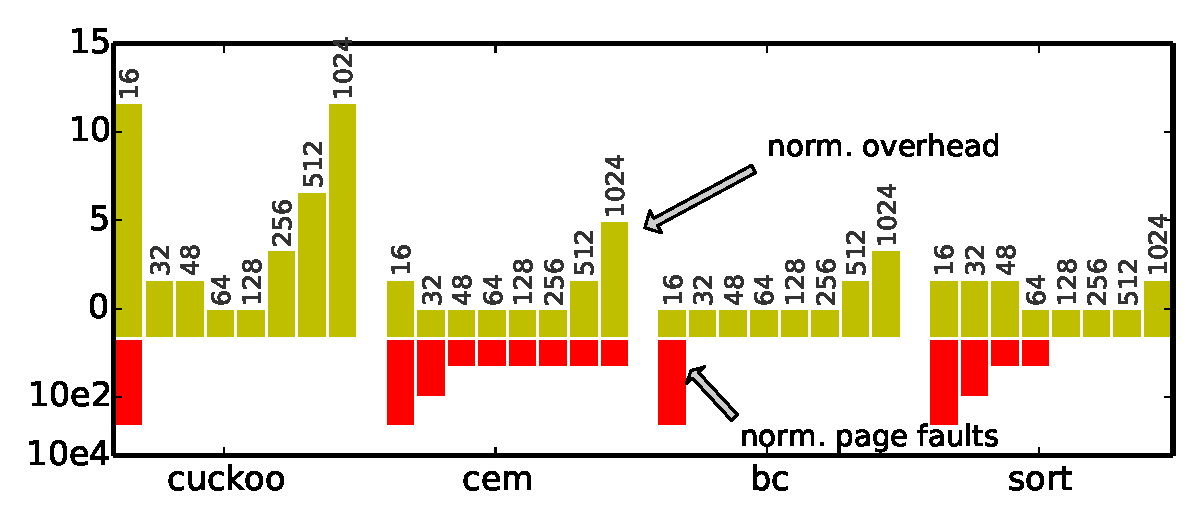
\includegraphics[width=\columnwidth]{figures/pagSizeOverhead}
	\caption{Initial figure about page size overhead. \todo{Figure placeholder---will be replaced with final one}{Amjad}}
	\label{fig:IPOSPerformance}
\end{figure}

\begin{figure}
	\centering
	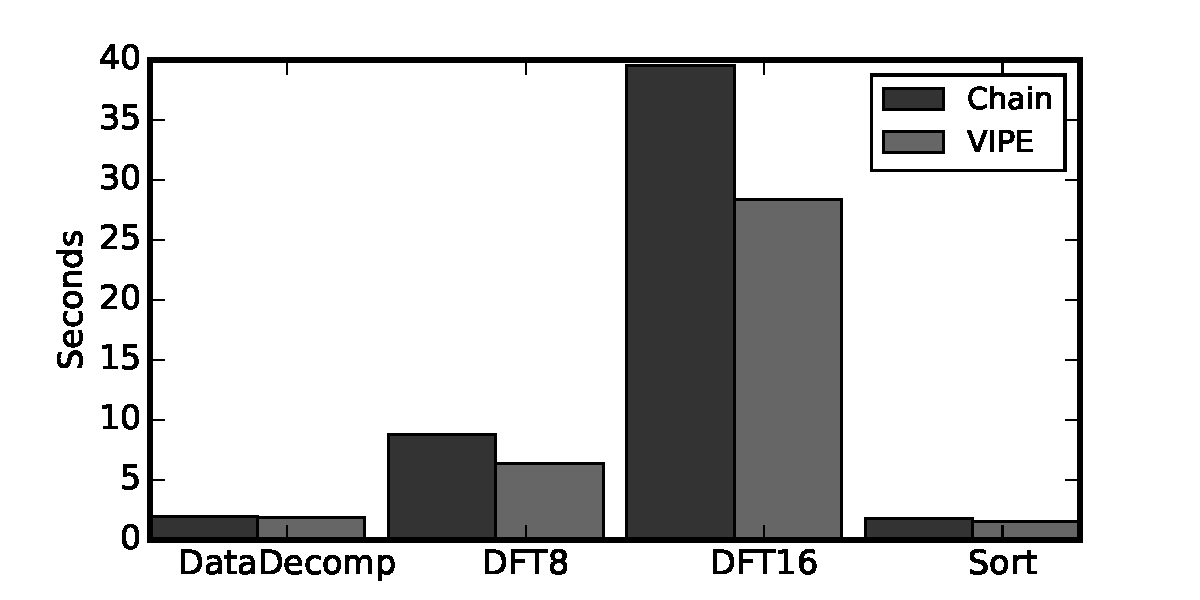
\includegraphics[width=\columnwidth]{figures/chain_vipe}
	\caption{Time to complete for a set of testing applications (refer to Table~\ref{table:benchmark_list}) using \sys versus Chain (no coalescing applied, fixed power supply). \todo{Figure placeholder---will be replaced with final one}{Amjad}}
	\label{fig:IPOSPerformance}
\end{figure}

Expected results:
\begin{itemize}
	\item Sensitivity plot---normalized page swapping cost ("bathtub" curve) in terms of execution time: compare against Chain and full double buffering approach; show number of page swaps---do the experiment for all applications
\end{itemize} 

\todo{Provide argument for page swapping using hardware support}{Brandon}

\subsubsection{Case Study}
\label{sec:case_study}

The final experiment assessing usefulness of \sys's use in real application. For this we have a implemented an battery-less wirelessly-powered sound detector as an example. To the best of our knowledge, this is the first case study that demonstrates a intermittently-powered system supplied by harvested energy at runtime, which continuously interacts with real-life signals. 

The application aims at detecting a specific tone in the audio signal (in the implementation: 1\,kHz) based on on-the-fly audio measurement. For this we have connected an analog MEMS microphone~\cite{microphone} output to AUX3 port of WISP\,5.1 (while the microphone was powered directly by WISP, which was then wirelessly power-supplied by the RFID reader). Audio signal is sampled by the microcontroller's ADC and passed to the FFT function (internal function of the TI's Digital Signal Processing library~\cite{ti_dsp}) to find a tone above a predefined threshold. The output of the detection is signalled by the WISP on-board LED. The video of demonstrating the working system is available via \url{https://link_to_a_video}.

Expected results:
\begin{itemize}
	\item Compare execution time: \sys against Chain for X\,s long audio signal detection at two antenna distances
	\item Make a video of the demonstration 
\end{itemize}
 
\todo{Check if we really need this application}{Brandon}
\todo{Provide results and text to this section---if time allows (this result is not critical)}{Amjad/Przemek}